\documentclass[english]{article}
\usepackage[T1]{fontenc}
\usepackage[latin9]{inputenc}
\usepackage[a4paper]{geometry}
\usepackage{amsmath}
\geometry{verbose,tmargin=2cm,bmargin=2cm,lmargin=2cm,rmargin=2cm}
\usepackage{graphicx}
%\usepackage[chapter]{algorithm}
\usepackage{algorithmic}
\usepackage{tabularx}
\usepackage{colortbl}
\usepackage{hhline}
\usepackage{pifont}
\usepackage{courier}
\usepackage{subcaption}
\usepackage[section]{placeins}
\newcommand{\norm}[1]{\left\lVert#1\right\rVert}

\DeclareMathOperator*{\argmin}{\arg\!\min}
\DeclareMathOperator*{\argmax}{\arg\!\max}

\makeatletter

%%%%%%%%%%%%%%%%%%%%%%%%%%%%%% LyX specific LaTeX commands.
%% Because html converters don't know tabularnewline
\providecommand{\tabularnewline}{\\}

\makeatother

\usepackage{babel}
\begin{document}

\title{Machine Learning for Computer Vision (EE5177) \\ Programming Assignment 4 : Logistic Regression and SVMs \\ Problem \#2}

\author{Akshit Kumar \\ \emph{EE14B127}}

\date{17th April 2017}

\maketitle
\tableofcontents{}

\section{Introduction}

\subsection{Goal}
The goal of the second question is to use SVMs to find hyperplane between linearly separable datapoints. The optional exercise requires the use of slack variables to find an optimum separating hyperplane between non-linearly separable data.
\subsection{Approach}
For getting the separating hyperplane, we formulate the dual of the SVM optimization problem and pass it through the convex optimization library called cvx.

\section{Linearly Separable Data}
\subsection{Bias-Variance Tradeoff}
As we can clearly see from the plots for different values of $\lambda$, the lower the value of $\lambda$, the more the data is overfitted and number of parameters are higher.Thus the variance increases and bias reduces. This is because the model starts to become more and more complicated with more non-zero values of $\alpha$. For $\lambda = 10$, we get 3 non-zero values of $\alpha$ which represents the number of support vectors used. For $\lambda = 1$, we get 32 non-zero values of $\alpha$ which represents the number of support vectors used.
We see that higher the value of $\lambda$, the more general the model is and fits better to the test data compared to the models due to lower value of $\lambda$.
\newline 
\newline
\textbf{
The optimal value of $\alpha$ vector obtained for $\lambda = 10$ has the following non-zero values : 102.769,11.018 and 91.974
}

\subsection{Contour Plots for different $\lambda$ values}

\begin{figure}[!htbp] 
\begin{subfigure}{0.48\textwidth}
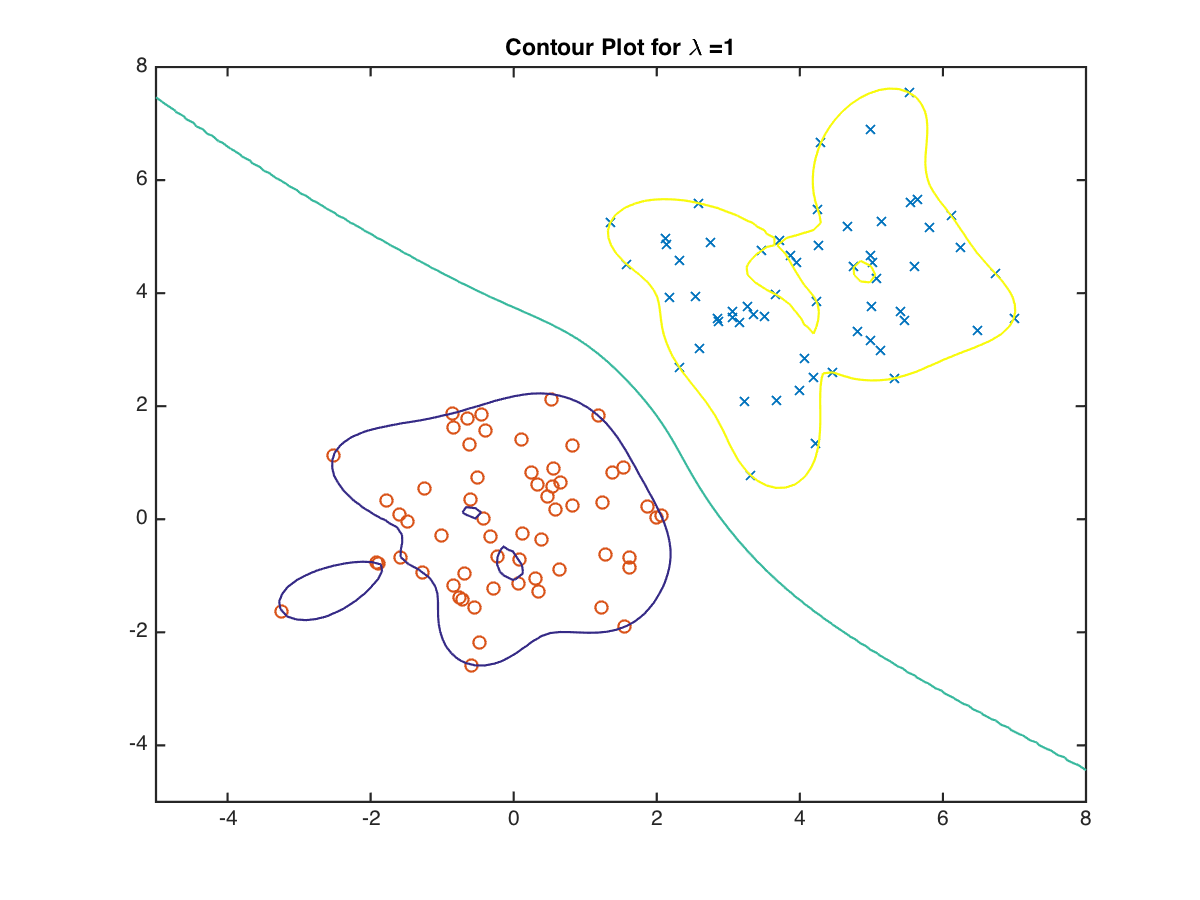
\includegraphics[width=\linewidth]{../plotLambda/plot_1}
\caption{Contour Plot for $\lambda$ = 1} 
\end{subfigure}\hspace*{\fill}
\begin{subfigure}{0.48\textwidth}
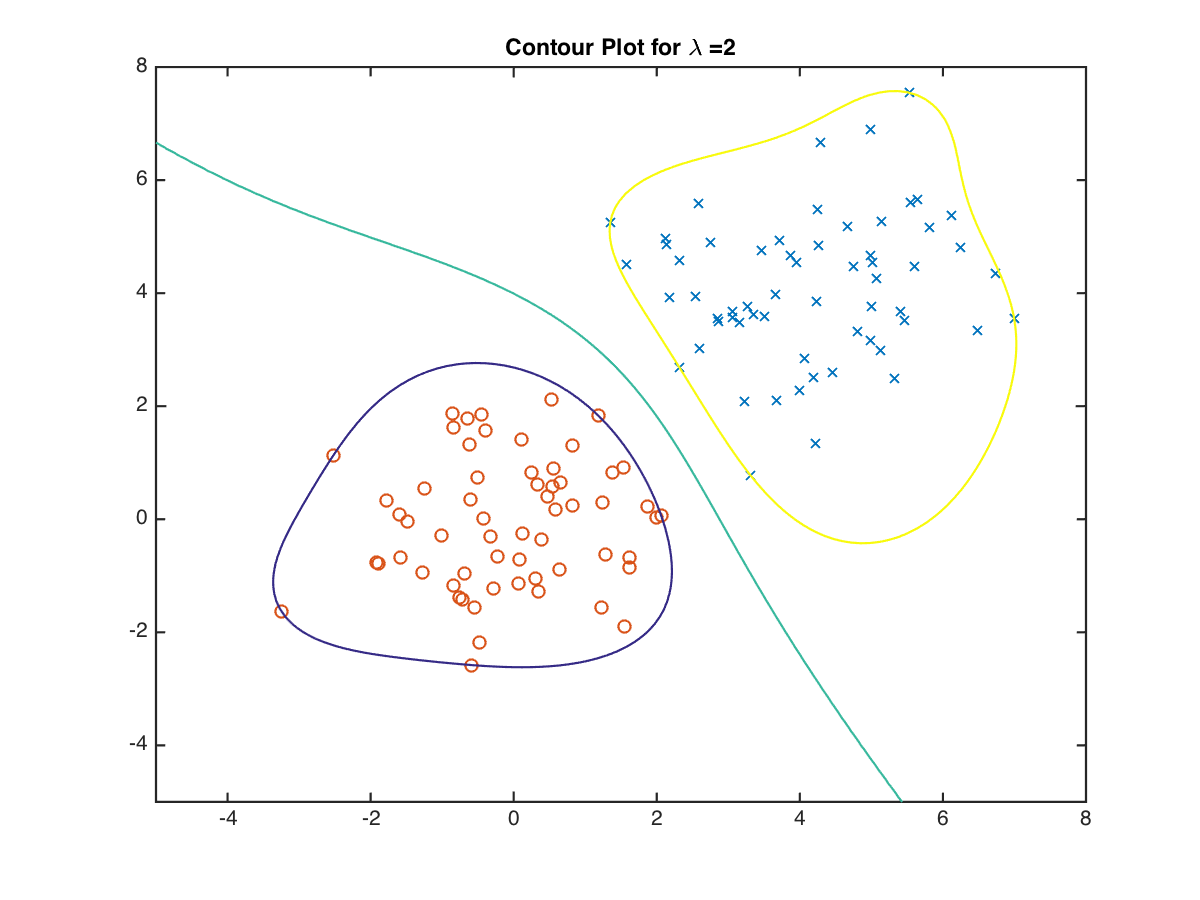
\includegraphics[width=\linewidth]{../plotLambda/plot_2}
\caption{Contour Plot for $\lambda$ = 2} \label{fig:b}
\end{subfigure}
%\caption{Con} \label{fig:1}
%\end{figure}

%\begin{figure}[!htbp] 
\begin{subfigure}{0.48\textwidth}
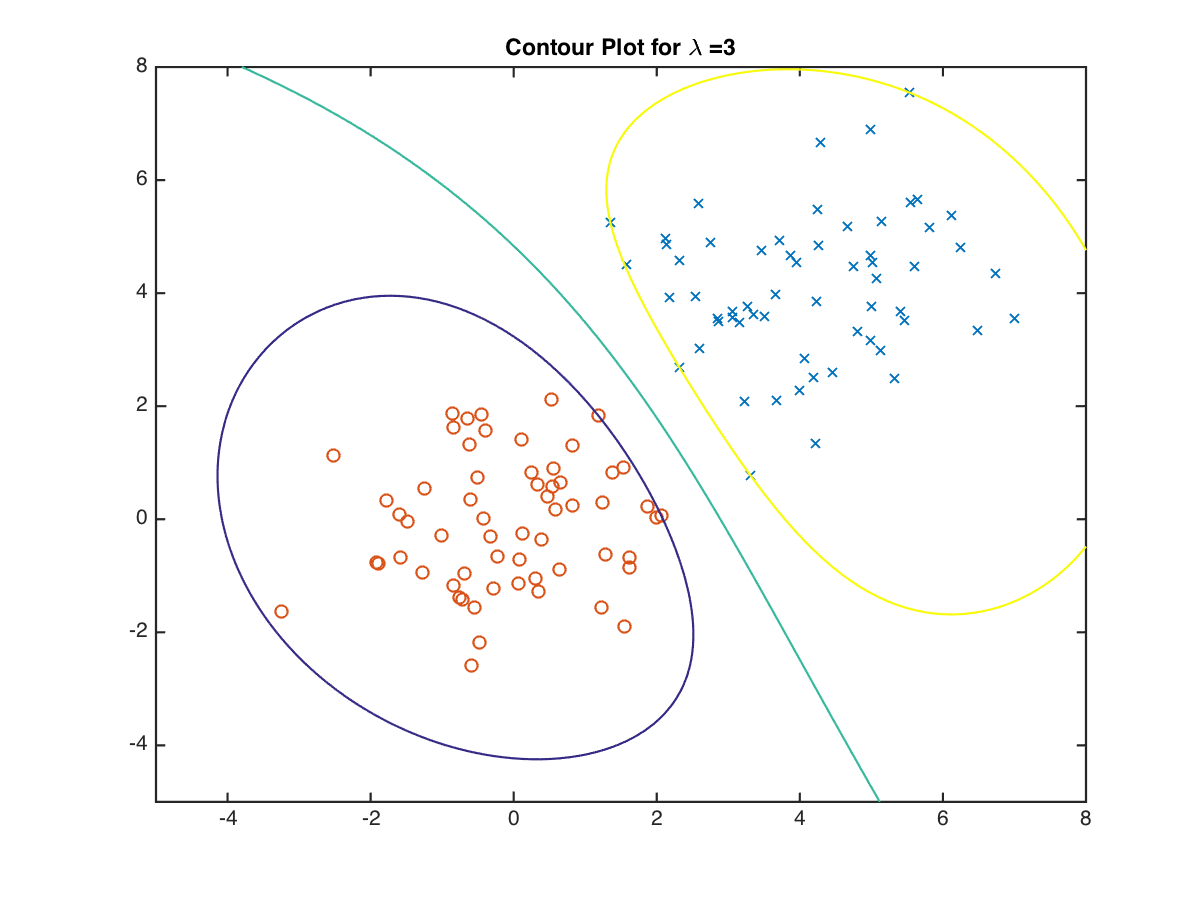
\includegraphics[width=\linewidth]{../plotLambda/plot_3}
\caption{Contour Plot for $\lambda$ = 3} 
\end{subfigure}\hspace*{\fill}
\begin{subfigure}{0.48\textwidth}
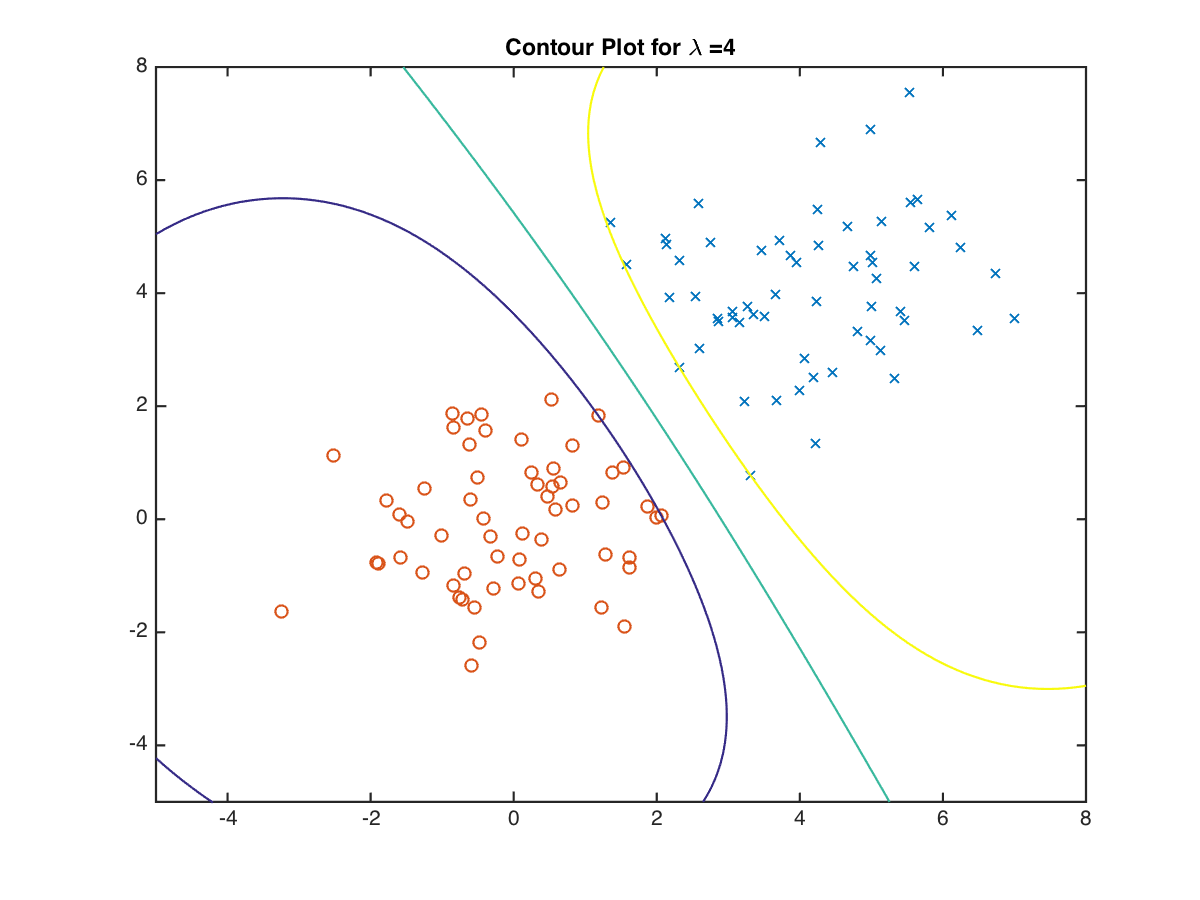
\includegraphics[width=\linewidth]{../plotLambda/plot_4}
\caption{Contour Plot for $\lambda$ = 4} \label{fig:b}
\end{subfigure}
\caption{Small value of $\lambda$} \label{fig:1}
\end{figure}

\begin{figure}[!htbp]
\begin{subfigure}{0.48\textwidth}
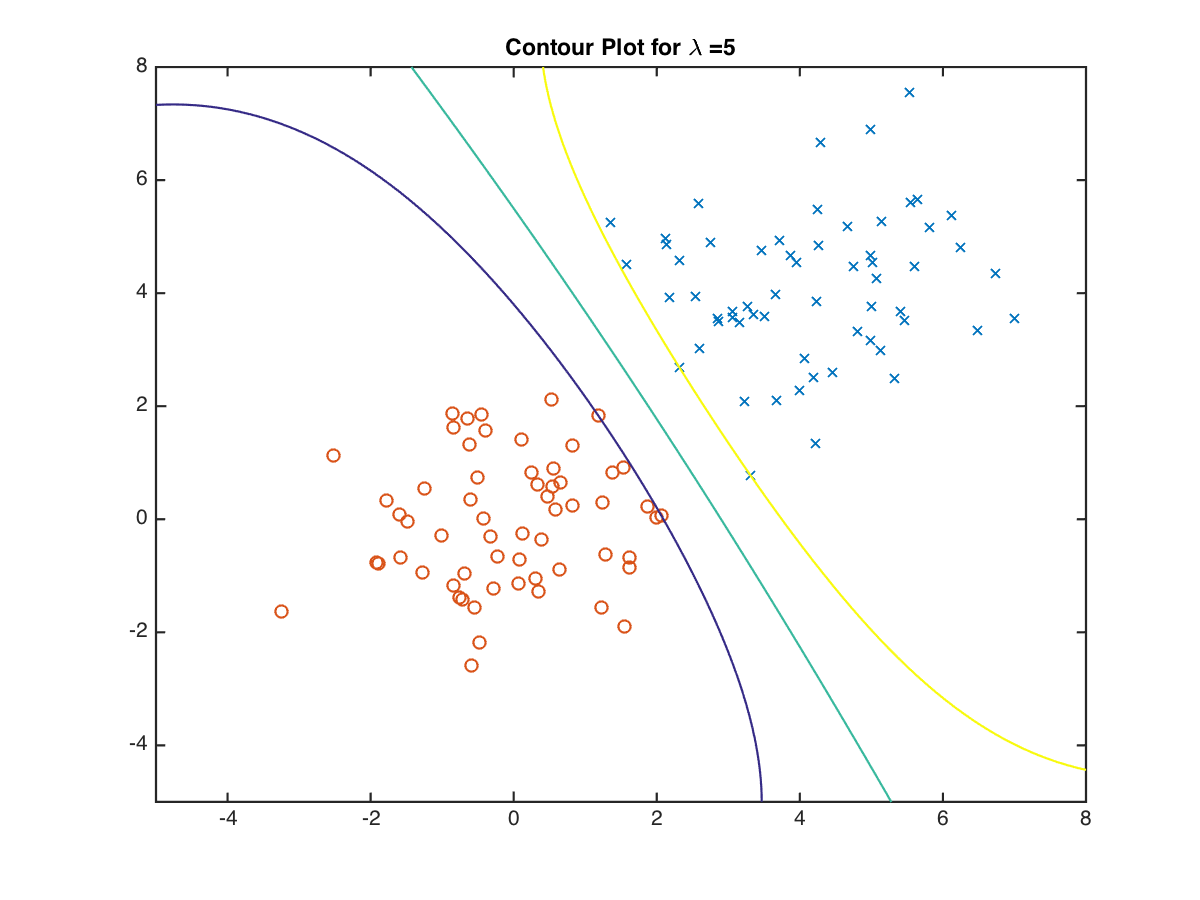
\includegraphics[width=\linewidth]{../plotLambda/plot_5}
\caption{Contour Plot for $\lambda$ = 5} 
\end{subfigure}\hspace*{\fill}
\begin{subfigure}{0.48\textwidth}
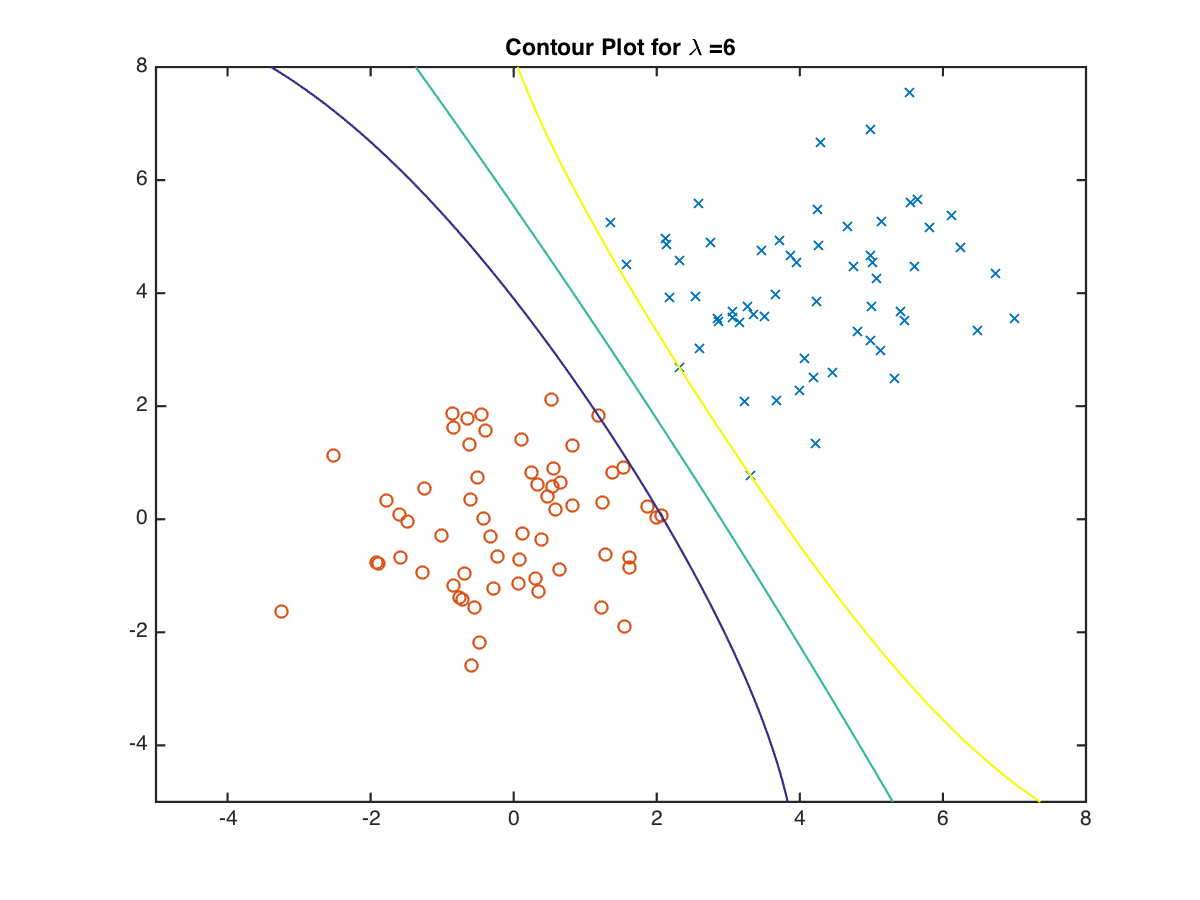
\includegraphics[width=\linewidth]{../plotLambda/plot_6}
\caption{Contour Plot for $\lambda$ = 6} \label{fig:b}
\end{subfigure}
\caption{Moderate value of $\lambda$} \label{fig:1}
\end{figure}

\begin{figure}[!htbp]
\begin{subfigure}{0.48\textwidth}
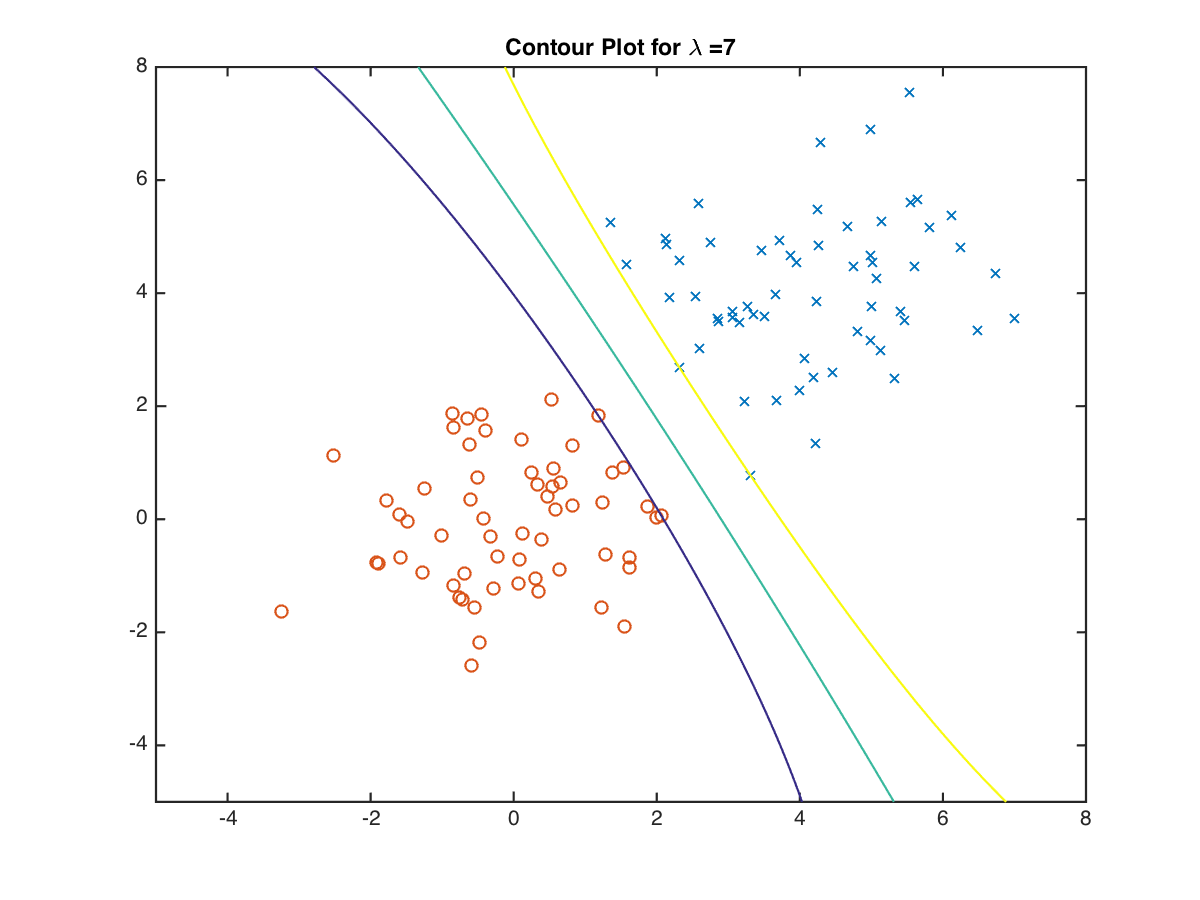
\includegraphics[width=\linewidth]{../plotLambda/plot_7}
\caption{Contour Plot for $\lambda$ = 7} 
\end{subfigure}\hspace*{\fill}
\begin{subfigure}{0.48\textwidth}
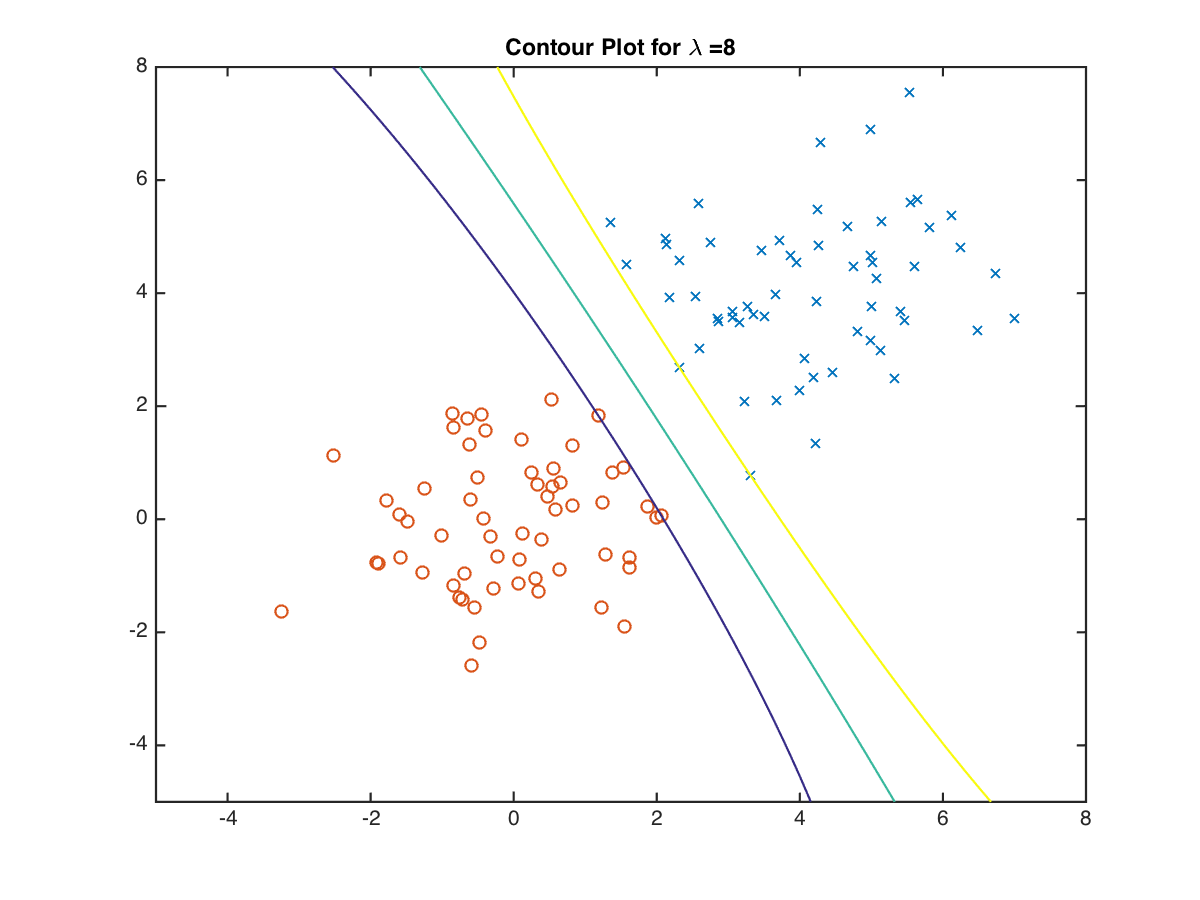
\includegraphics[width=\linewidth]{../plotLambda/plot_8}
\caption{Contour Plot for $\lambda$ = 8} \label{fig:b}
\end{subfigure}

%\end{figure}


\begin{subfigure}{0.48\textwidth}
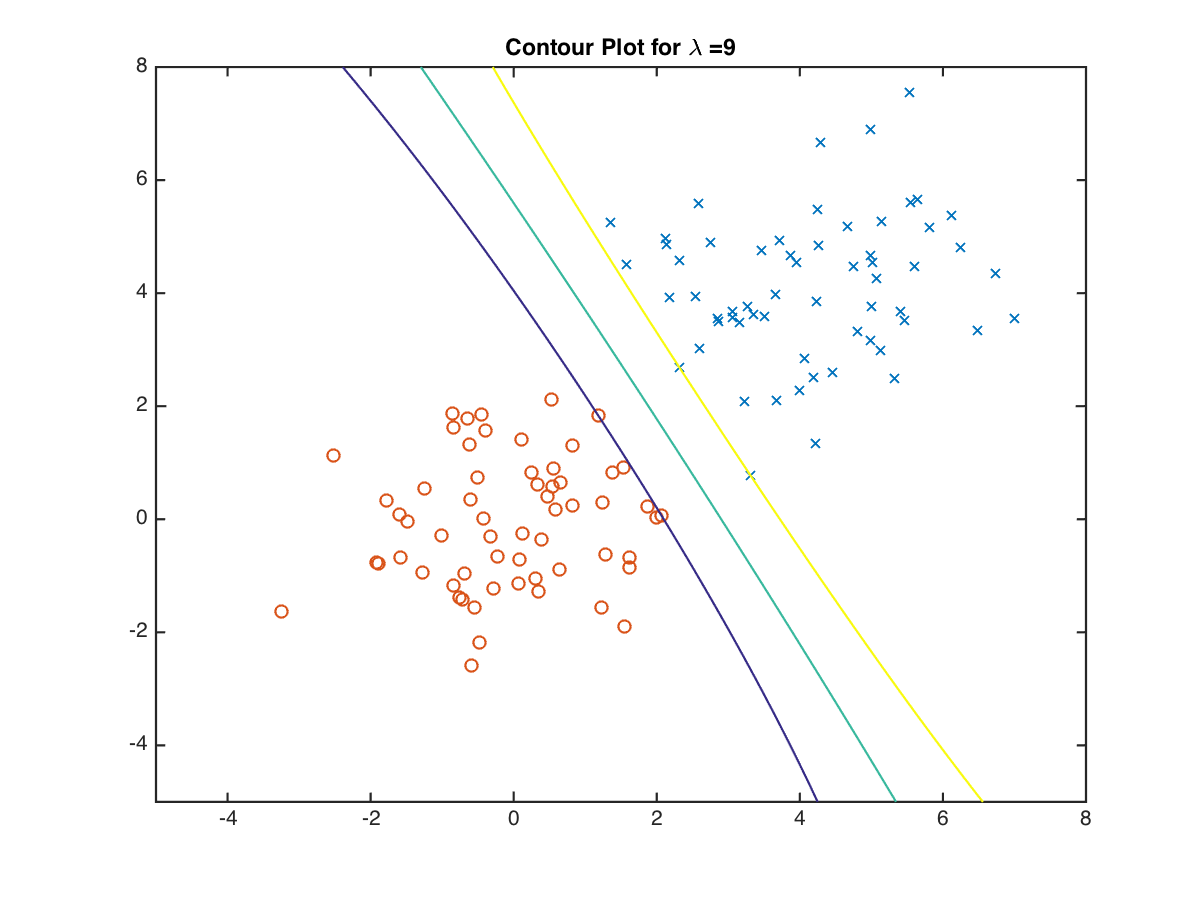
\includegraphics[width=\linewidth]{../plotLambda/plot_9}
\caption{Contour Plot for $\lambda$ = 9} 
\end{subfigure}\hspace*{\fill}
\begin{subfigure}{0.48\textwidth}
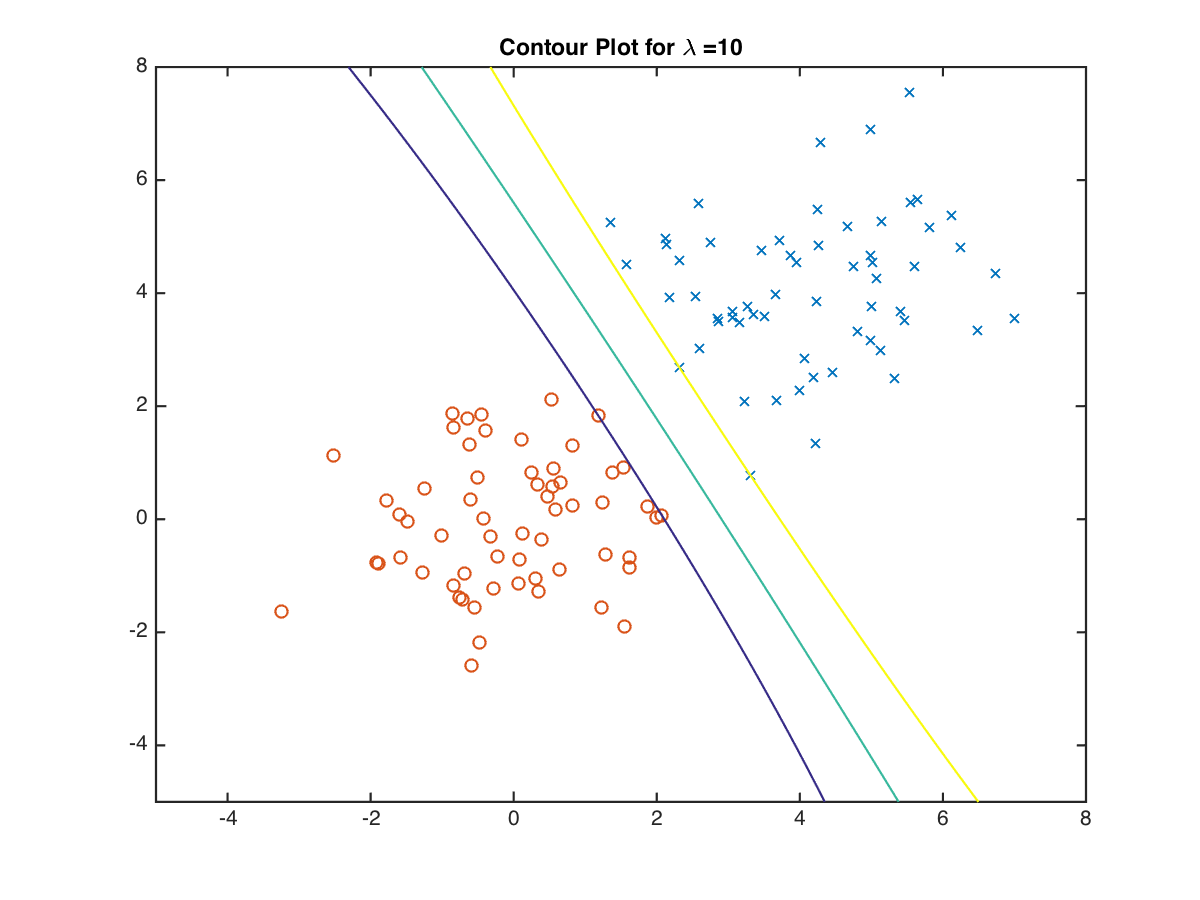
\includegraphics[width=\linewidth]{../plotLambda/plot_10}
\caption{Contour Plot for $\lambda$ = 10} \label{fig:b}
\end{subfigure}
\caption{Large value of $\lambda$} \label{fig:1}
\end{figure}



\subsection{Required Iteration Data for $\lambda$ = 1}
\begin{itemize}
	\item Number of iterations : 23
	\item  norm(X), norm(y), norm(Z) = 1.2e+01, 9.1e+00, 1.2e+01
 	\item norm(A), norm(b), norm(C) = 1.7e+01, 1.2e+01, 2.0e+00
 	\item Total CPU time(secs) : 0.68
 	\item Optimal value for $\alpha$ :-7.83293
 \end{itemize}

 \subsection{Required Iteration Data for $\lambda$ = 10}
\begin{itemize}
	\item Number of iterations : 15
	\item  norm(X), norm(y), norm(Z) = 1.5e+02, 1.1e+02, 1.5e+02
 	\item norm(A), norm(b), norm(C) = 9.7e+00, 2.0e+00, 1.2e+01
 	\item Total CPU time(secs) : 0.40
 	\item Optimal value for $\alpha$ : -102.882
 \end{itemize}

\section{Non Linearly Separable Data : Use of Slack Variables}
\subsection{Goal}
In this part of the problem, we modify the above used convex optimization problem by introducing slack variables to classify data which is non linearly separable. 
\subsection{Approach}
Since the dataset is not linearly separable, we are required to misclassify certain points to get an optimal solution. Hence we add slack variables to generate the separating hyperplane.

 \subsection{Required Iteration Data for $\lambda$ = 10 and C = 1}
\begin{itemize}
	\item Number of iterations : 18
	\item  norm(X), norm(y), norm(Z) = 2.0e+01, 7.6e+00, 1.2e+01
 	\item norm(A), norm(b), norm(C) = 1.8e+01, 1.2e+01, 1.2e+01
 	\item Total CPU time(secs) : 0.55 
 	\item Optimal value for $\alpha$ : -28.1351
 \end{itemize}

  \subsection{Required Iteration Data for $\lambda$ = 10 and C = 100000}
\begin{itemize}
	\item Number of iterations : 25
	\item  norm(X), norm(y), norm(Z) = 3.5e+04, 2.6e+05, 1.1e+06
 	\item  norm(A), norm(b), norm(C) = 1.8e+01, 1.2e+01, 1.1e+06
 	\item Total CPU time(secs) : 0.70
 	\item Optimal value for $\alpha$ : -674174
 \end{itemize}

\subsection{Varying C}
The parameter C controls how much we penalise the objective function for misclassifying a data point. For large values of C, the model would not be willing to misclassify any data point. For small values of C, the model would misclassify data very easily.
\newline
In case of a dataset which is not linearly separable, it is better to not overfit the data and use smaller value of slack. This should capture the general trend in the data and overfit the same.
\subsection{Plots for various values of C}
\begin{figure}[!htbp]
\begin{subfigure}{0.48\textwidth}
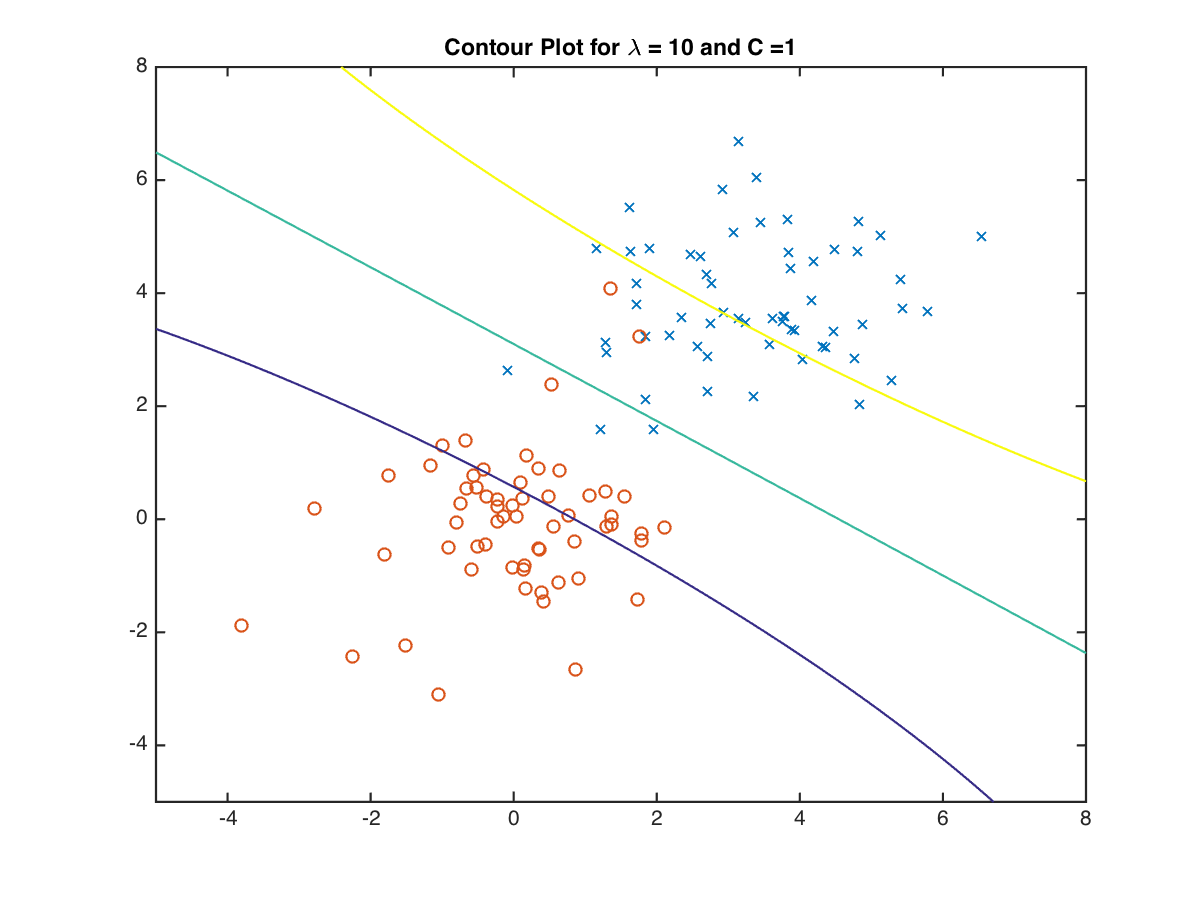
\includegraphics[width=\linewidth]{../plotC/plot_C_1}
\caption{Contour Plot for $\lambda$ = 10 and C = 1} 
\end{subfigure}\hspace*{\fill}
\begin{subfigure}{0.48\textwidth}
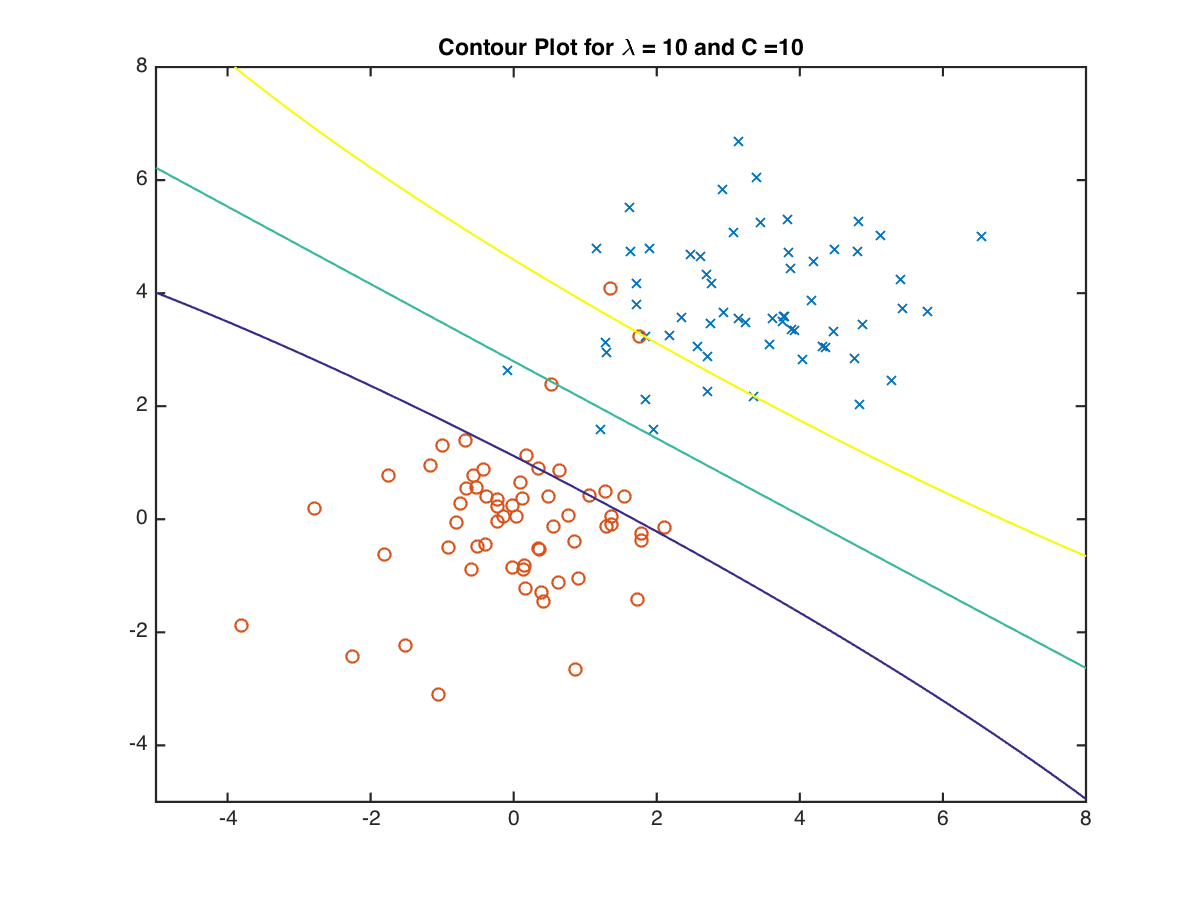
\includegraphics[width=\linewidth]{../plotC/plot_C_10}
\caption{Contour Plot for $\lambda$ = 10 and C = 10} \label{fig:b}
\end{subfigure}

%\end{figure}


\begin{subfigure}{0.48\textwidth}
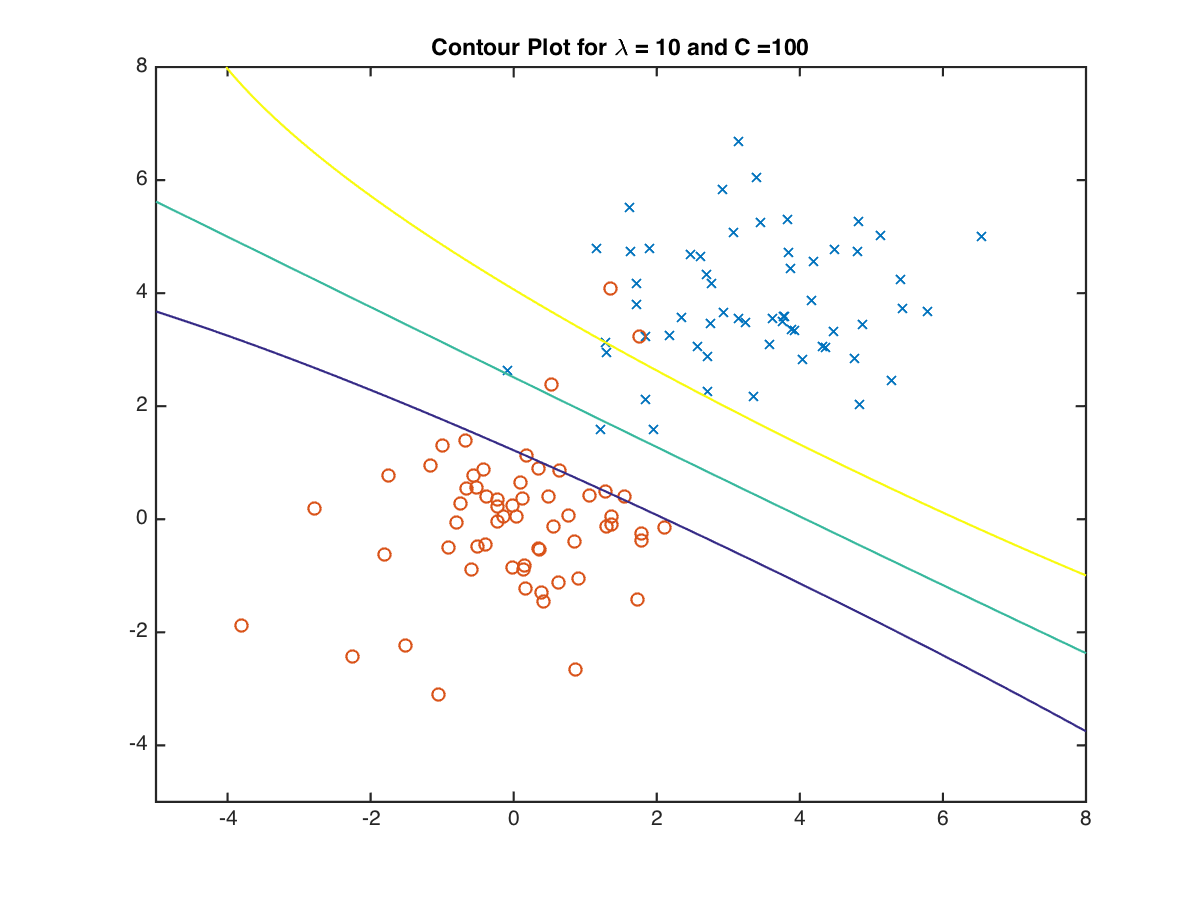
\includegraphics[width=\linewidth]{../plotC/plot_C_100}
\caption{Contour Plot for $\lambda$ = 10 and C = 100} 
\end{subfigure}\hspace*{\fill}
\begin{subfigure}{0.48\textwidth}
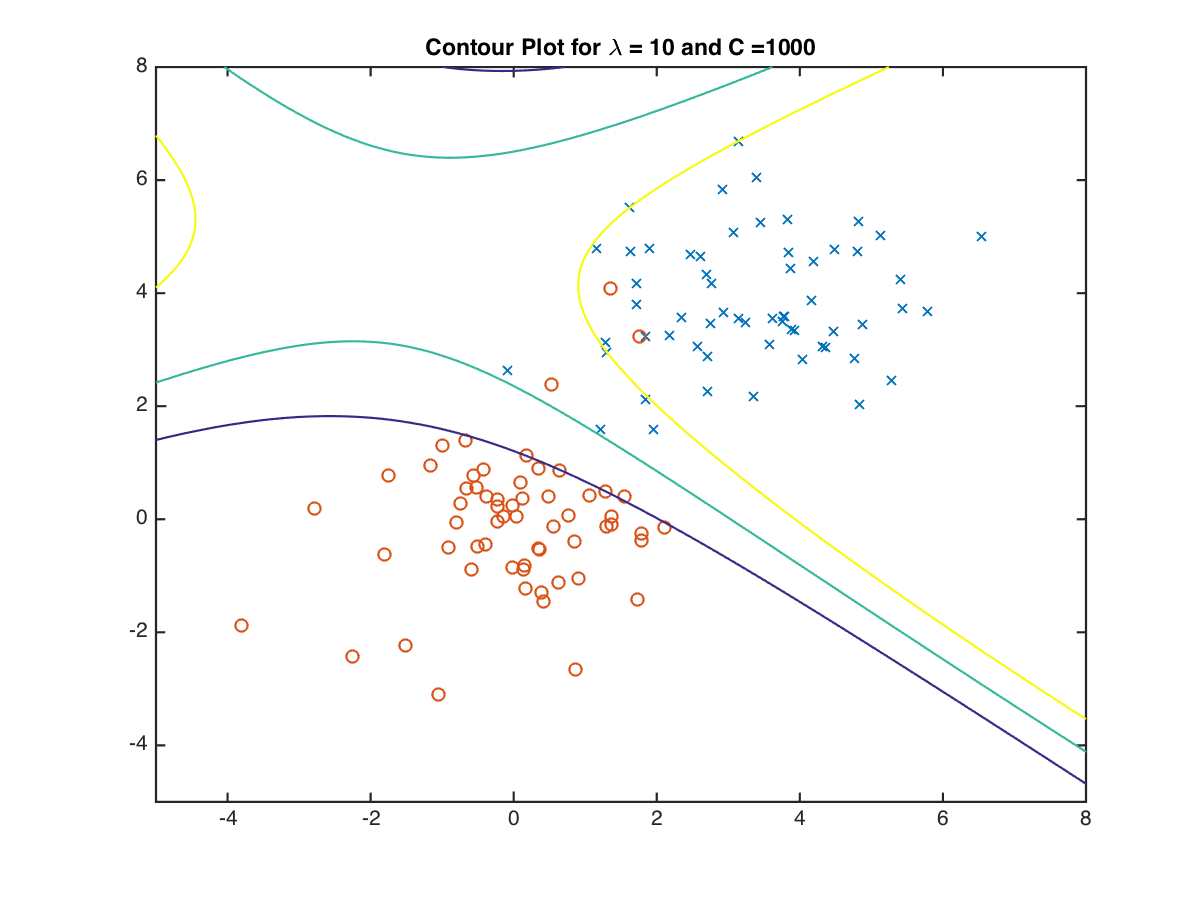
\includegraphics[width=\linewidth]{../plotC/plot_C_1000}
\caption{Contour Plot for $\lambda$ = 10 and C = 1000} \label{fig:b}
\end{subfigure}

\begin{subfigure}{0.48\textwidth}
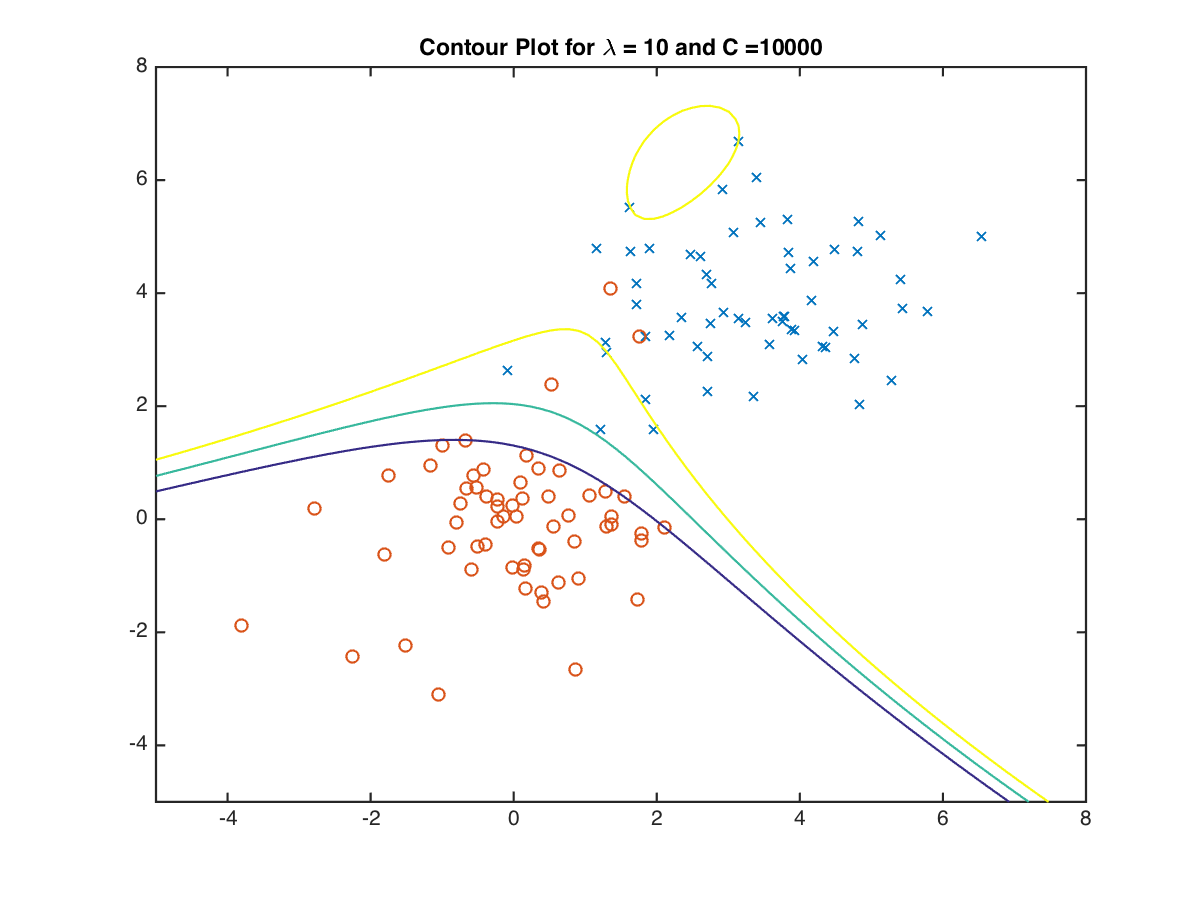
\includegraphics[width=\linewidth]{../plotC/plot_C_10000}
\caption{Contour Plot for $\lambda$ = 10 and C = 10000} 
\end{subfigure}\hspace*{\fill}
\begin{subfigure}{0.48\textwidth}
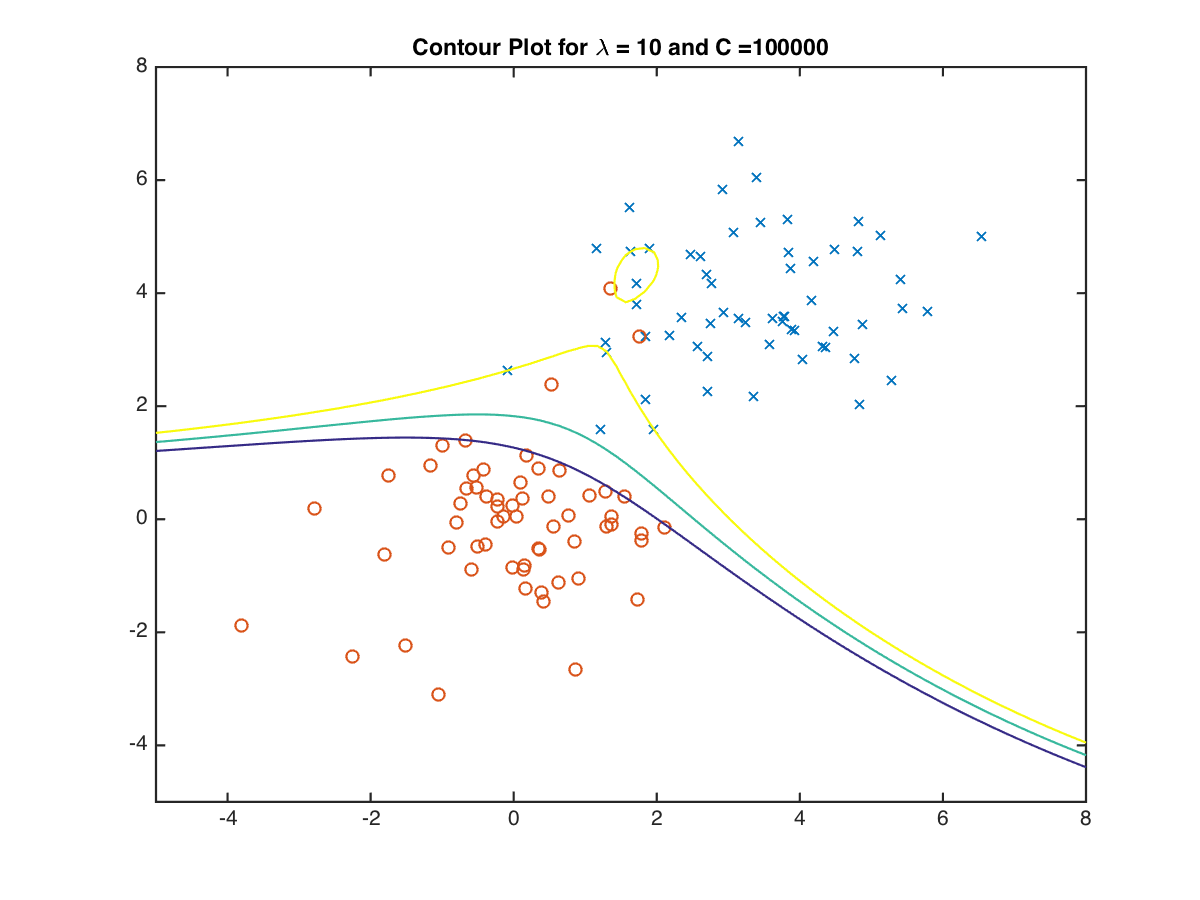
\includegraphics[width=\linewidth]{../plotC/plot_C_100000}
\caption{Contour Plot for $\lambda$ = 10 and C = 100000} \label{fig:b}
\end{subfigure}

\end{figure}

\end{document}



